\documentclass[14pt]{extbook}
\usepackage{multicol, enumerate, enumitem, hyperref, color, soul, setspace, parskip, fancyhdr} %General Packages
\usepackage{amssymb, amsthm, amsmath, latexsym, units, mathtools} %Math Packages
\everymath{\displaystyle} %All math in Display Style
% Packages with additional options
\usepackage[headsep=0.5cm,headheight=12pt, left=1 in,right= 1 in,top= 1 in,bottom= 1 in]{geometry}
\usepackage[usenames,dvipsnames]{xcolor}
\usepackage{dashrule}  % Package to use the command below to create lines between items
\newcommand{\litem}[1]{\item#1\hspace*{-1cm}\rule{\textwidth}{0.4pt}}
\pagestyle{fancy}
\lhead{Progress Quiz 5}
\chead{}
\rhead{Version A}
\lfoot{8497-6012}
\cfoot{}
\rfoot{Summer C 2021}
\begin{document}

\begin{enumerate}
\litem{
Solve the quadratic equation below. Then, choose the intervals that the solutions belong to, with $x_1 \leq x_2$ (if they exist).\[ -14x^{2} -13 x + 7 = 0 \]\begin{enumerate}[label=\Alph*.]
\item \( x_1 \in [-25.11, -23.76] \text{ and } x_2 \in [22.6, 25.7] \)
\item \( x_1 \in [-0.49, -0.3] \text{ and } x_2 \in [1.1, 3.2] \)
\item \( x_1 \in [-2.86, -1.21] \text{ and } x_2 \in [-0.2, 0.7] \)
\item \( x_1 \in [-6.36, -4.31] \text{ and } x_2 \in [17.4, 19.1] \)
\item \( \text{There are no Real solutions.} \)

\end{enumerate} }
\litem{
Solve the quadratic equation below. Then, choose the intervals that the solutions $x_1$ and $x_2$ belong to, with $x_1 \leq x_2$.\[ 25x^{2} -15 x -54 = 0 \]\begin{enumerate}[label=\Alph*.]
\item \( x_1 \in [-6.12, -5.4] \text{ and } x_2 \in [0.13, 0.59] \)
\item \( x_1 \in [-0.76, -0.47] \text{ and } x_2 \in [3.58, 3.93] \)
\item \( x_1 \in [-4.04, -3.17] \text{ and } x_2 \in [0.47, 0.87] \)
\item \( x_1 \in [-1.58, -0.64] \text{ and } x_2 \in [1.69, 1.98] \)
\item \( x_1 \in [-30.39, -29.06] \text{ and } x_2 \in [44.7, 45.48] \)

\end{enumerate} }
\litem{
Write the equation of the graph presented below in the form $f(x)=ax^2+bx+c$, assuming  $a=1$ or $a=-1$. Then, choose the intervals that $a, b,$ and $c$ belong to.
\begin{center}
    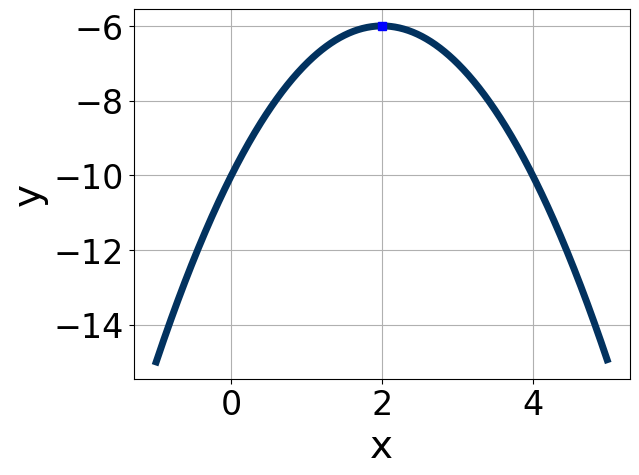
\includegraphics[width=0.5\textwidth]{../Figures/quadraticGraphToEquationCopyA.png}
\end{center}
\begin{enumerate}[label=\Alph*.]
\item \( a \in [-1, 0], \hspace*{5mm} b \in [3, 6], \text{ and } \hspace*{5mm} c \in [-12, -9] \)
\item \( a \in [1, 2], \hspace*{5mm} b \in [-6, -1], \text{ and } \hspace*{5mm} c \in [-2, 0] \)
\item \( a \in [-1, 0], \hspace*{5mm} b \in [-6, -1], \text{ and } \hspace*{5mm} c \in [-12, -9] \)
\item \( a \in [-1, 0], \hspace*{5mm} b \in [-6, -1], \text{ and } \hspace*{5mm} c \in [1, 6] \)
\item \( a \in [1, 2], \hspace*{5mm} b \in [3, 6], \text{ and } \hspace*{5mm} c \in [-2, 0] \)

\end{enumerate} }
\litem{
Factor the quadratic below. Then, choose the intervals that contain the constants in the form $(ax+b)(cx+d); b \leq d.$\[ 24x^{2} +10 x -25 \]\begin{enumerate}[label=\Alph*.]
\item \( a \in [5.71, 7.84], \hspace*{5mm} b \in [-9, -3], \hspace*{5mm} c \in [3.01, 4.8], \text{ and } \hspace*{5mm} d \in [2, 9] \)
\item \( a \in [1.39, 2.74], \hspace*{5mm} b \in [-9, -3], \hspace*{5mm} c \in [11.17, 12.67], \text{ and } \hspace*{5mm} d \in [2, 9] \)
\item \( a \in [-0.34, 1.88], \hspace*{5mm} b \in [-20, -15], \hspace*{5mm} c \in [0.8, 1.94], \text{ and } \hspace*{5mm} d \in [27, 31] \)
\item \( a \in [10.73, 12.47], \hspace*{5mm} b \in [-9, -3], \hspace*{5mm} c \in [1.86, 2.49], \text{ and } \hspace*{5mm} d \in [2, 9] \)
\item \( \text{None of the above.} \)

\end{enumerate} }
\litem{
Solve the quadratic equation below. Then, choose the intervals that the solutions $x_1$ and $x_2$ belong to, with $x_1 \leq x_2$.\[ 10x^{2} -53 x + 36 = 0 \]\begin{enumerate}[label=\Alph*.]
\item \( x_1 \in [0.82, 0.99] \text{ and } x_2 \in [3.18, 4.08] \)
\item \( x_1 \in [0.55, 0.84] \text{ and } x_2 \in [4.16, 4.94] \)
\item \( x_1 \in [0.35, 0.47] \text{ and } x_2 \in [8.74, 9.12] \)
\item \( x_1 \in [8, 8.12] \text{ and } x_2 \in [44.8, 45.7] \)
\item \( x_1 \in [1.46, 1.63] \text{ and } x_2 \in [1.24, 2.58] \)

\end{enumerate} }
\litem{
Solve the quadratic equation below. Then, choose the intervals that the solutions belong to, with $x_1 \leq x_2$ (if they exist).\[ 20x^{2} -13 x -9 = 0 \]\begin{enumerate}[label=\Alph*.]
\item \( x_1 \in [-29.78, -29.25] \text{ and } x_2 \in [28.5, 30.7] \)
\item \( x_1 \in [-1.64, -0.95] \text{ and } x_2 \in [0.1, 0.9] \)
\item \( x_1 \in [-0.54, -0.12] \text{ and } x_2 \in [0.6, 1.5] \)
\item \( x_1 \in [-8.61, -7.69] \text{ and } x_2 \in [19.8, 22.5] \)
\item \( \text{There are no Real solutions.} \)

\end{enumerate} }
\litem{
Factor the quadratic below. Then, choose the intervals that contain the constants in the form $(ax+b)(cx+d); b \leq d.$\[ 54x^{2} +33 x -10 \]\begin{enumerate}[label=\Alph*.]
\item \( a \in [-0.4, 1.2], \hspace*{5mm} b \in [-14, -11], \hspace*{5mm} c \in [0.3, 1.3], \text{ and } \hspace*{5mm} d \in [41, 54] \)
\item \( a \in [17.6, 19], \hspace*{5mm} b \in [-3, 3], \hspace*{5mm} c \in [1.6, 3.3], \text{ and } \hspace*{5mm} d \in [5, 15] \)
\item \( a \in [8.4, 10.1], \hspace*{5mm} b \in [-3, 3], \hspace*{5mm} c \in [5.5, 7], \text{ and } \hspace*{5mm} d \in [5, 15] \)
\item \( a \in [1.3, 5.3], \hspace*{5mm} b \in [-3, 3], \hspace*{5mm} c \in [16.4, 21.1], \text{ and } \hspace*{5mm} d \in [5, 15] \)
\item \( \text{None of the above.} \)

\end{enumerate} }
\litem{
Graph the equation below.\[ f(x) = -(x-3)^2 - 16 \]\begin{enumerate}[label=\Alph*.]
\begin{multicols}{2}\item 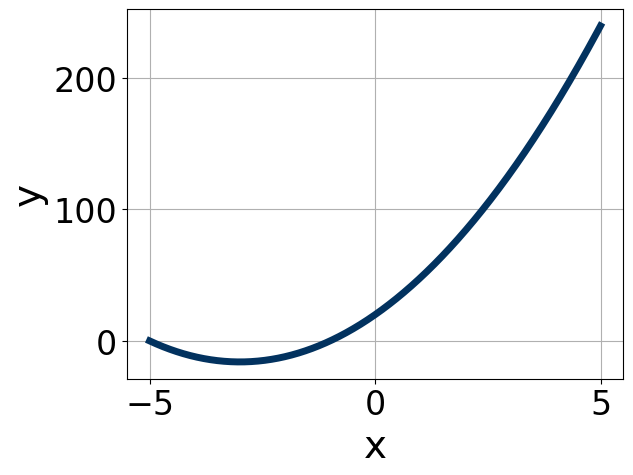
\includegraphics[width = 0.3\textwidth]{../Figures/quadraticEquationToGraphCopyAA.png}\item 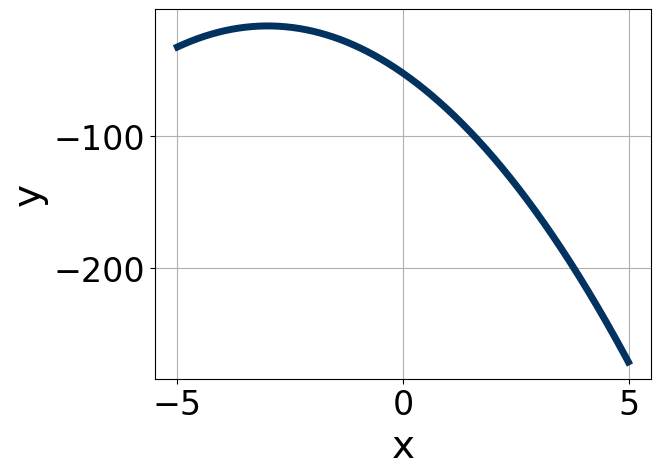
\includegraphics[width = 0.3\textwidth]{../Figures/quadraticEquationToGraphCopyBA.png}\item 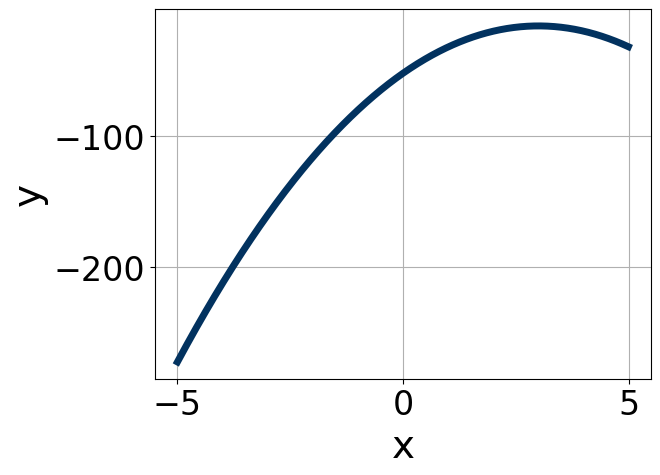
\includegraphics[width = 0.3\textwidth]{../Figures/quadraticEquationToGraphCopyCA.png}\item 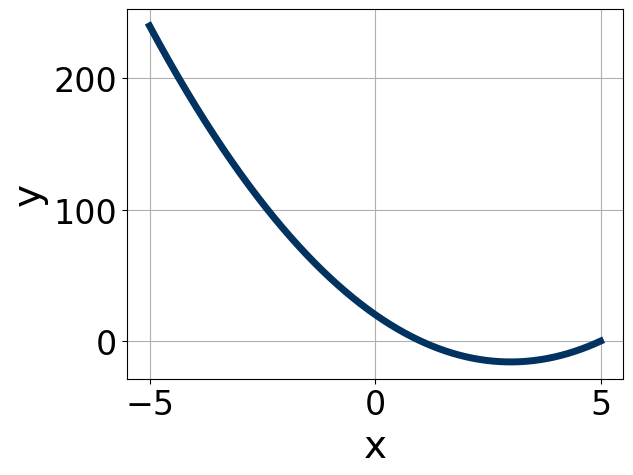
\includegraphics[width = 0.3\textwidth]{../Figures/quadraticEquationToGraphCopyDA.png}\end{multicols}\item None of the above.
\end{enumerate} }
\litem{
Write the equation of the graph presented below in the form $f(x)=ax^2+bx+c$, assuming  $a=1$ or $a=-1$. Then, choose the intervals that $a, b,$ and $c$ belong to.
\begin{center}
    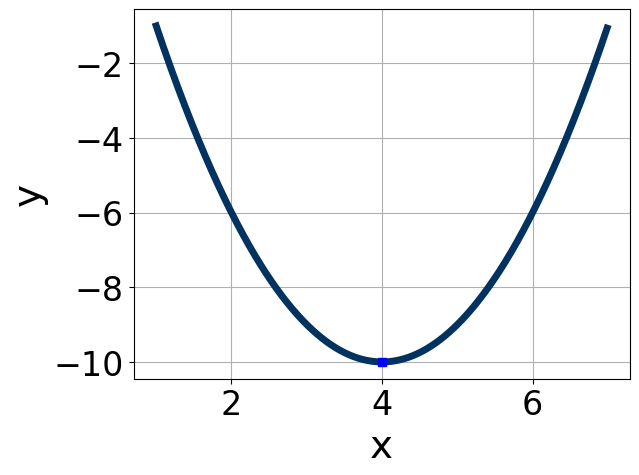
\includegraphics[width=0.5\textwidth]{../Figures/quadraticGraphToEquationA.png}
\end{center}
\begin{enumerate}[label=\Alph*.]
\item \( a \in [0.6, 1.5], \hspace*{5mm} b \in [-11, -6], \text{ and } \hspace*{5mm} c \in [5, 8] \)
\item \( a \in [-1.5, -0.1], \hspace*{5mm} b \in [-11, -6], \text{ and } \hspace*{5mm} c \in [-27, -25] \)
\item \( a \in [0.6, 1.5], \hspace*{5mm} b \in [8, 11], \text{ and } \hspace*{5mm} c \in [5, 8] \)
\item \( a \in [-1.5, -0.1], \hspace*{5mm} b \in [8, 11], \text{ and } \hspace*{5mm} c \in [-27, -25] \)
\item \( a \in [0.6, 1.5], \hspace*{5mm} b \in [8, 11], \text{ and } \hspace*{5mm} c \in [25, 28] \)

\end{enumerate} }
\litem{
Graph the equation below.\[ f(x) = -(x-4)^2 - 13 \]\begin{enumerate}[label=\Alph*.]
\begin{multicols}{2}\item 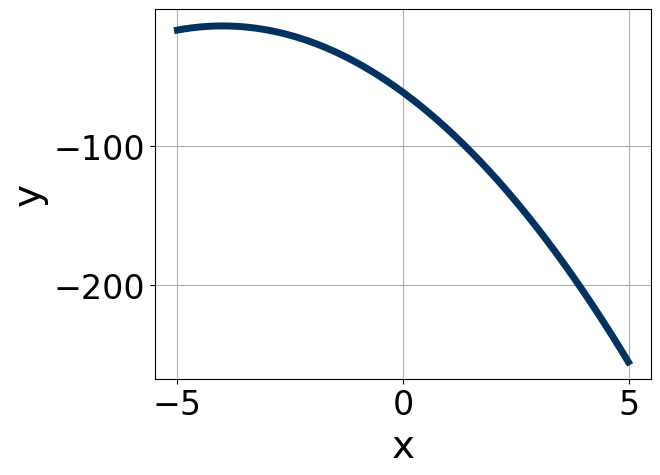
\includegraphics[width = 0.3\textwidth]{../Figures/quadraticEquationToGraphAA.png}\item 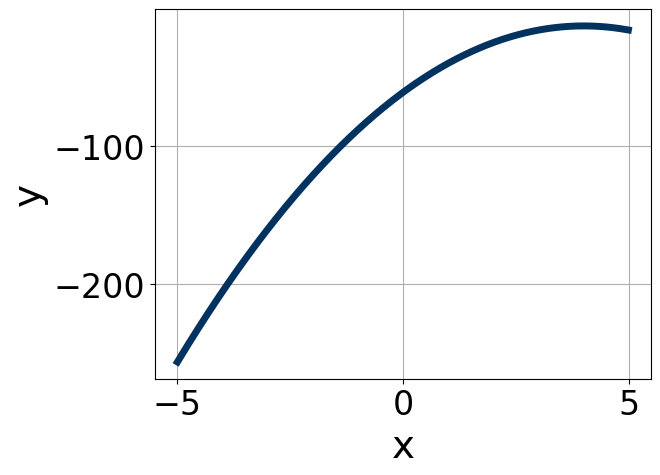
\includegraphics[width = 0.3\textwidth]{../Figures/quadraticEquationToGraphBA.png}\item 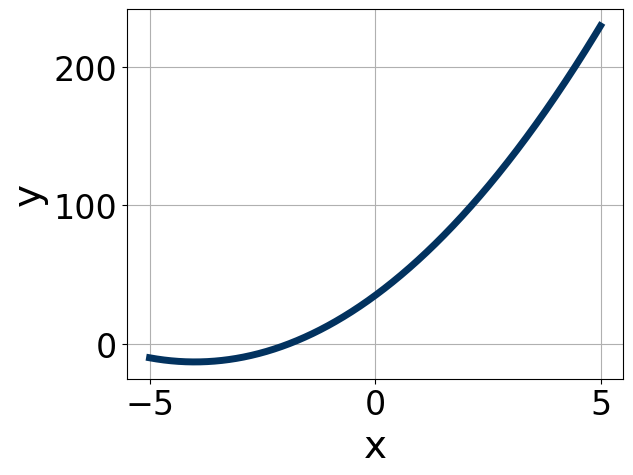
\includegraphics[width = 0.3\textwidth]{../Figures/quadraticEquationToGraphCA.png}\item 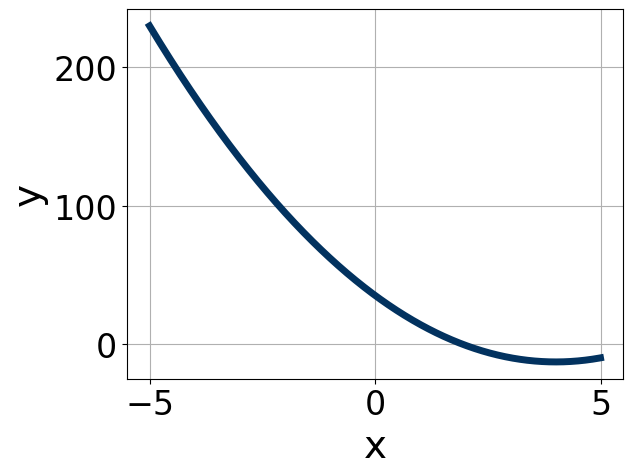
\includegraphics[width = 0.3\textwidth]{../Figures/quadraticEquationToGraphDA.png}\end{multicols}\item None of the above.
\end{enumerate} }
\end{enumerate}

\end{document}